\chapter{Introduction}
\setstretch{\lspac}

It has been suggested that the processes that drive horizontal (tangential) and vertical (radial) development of the cerebral cortex are separate from each other \citep{Rakic1988}. Variations on these would result, respectively, in variations on the extent of cortical surface area and on the thickness of the cortical mantle. Through the use of genetically informative samples, it has been demonstrated these two processes are indeed uncorrelated genetically \citep{Panizzon2009, Winkler2010} and are each influenced by regionally distinct genetic factors \citep{Schmitt2008,Rimol2010a}. Moreover, it is variation on surface area that explains most of the variation observed in the amount of gray matter assessed with methods that only measure volume, such as voxel-based morphometry \citep{Winkler2010, Rimol2012}.

These findings give prominence to the use of surface area alongside cortical thickness in studies of brain morphology and, and its interaction with brain function. However, cortical surface area been measured only over gross regions or approached indirectly via comparisons with a standard brain. Of studies using the latter, few that have used area measurements on every point of the cortex (vertexwise) and have offered detailed insight on the exact procedures used for this assessment. Some studies described their methods in terms of ``expansion/contraction'', often using different definitions of what expansion or contraction would be. By 2011, various impromptu approaches had been considered, for example:

\begin{itemize}
\item[--] \citet{Lyttelton2009}: The authors describe that the asymmetry measurement is the logarithm of the ratio of the area per vertex of left and right hemispheres. Expansion or contraction are in relation to the contralateral hemisphere.
\item[--] \citet{Joyner2009}: After a brief description of the method of measurement, the authors state that ``(\ldots) this provides point-by-point estimates of the relative areal expansion or compression of each location in atlas space.'' Expansion/contraction are relative to the chosen template.
\item[--] \citet{Sun2009a}: The authors state that ``The distance between a center position of the brain (\ldots) and each brain surface point was calculated (\ldots). The difference of the above radial distances between the follow-up and baseline brain surfaces (\ldots) was defined as brain surface contraction''. Under this definition, not only contraction refers to an initial point in time, but it also refers not to a bidimensional feature, and instead to a linear distance between each point in the surface and a given central point in the brain.
\item[--] \citet{Sun2009}: The authors state that ``The distance between two brain surfaces [\emph{i.e. inner skull and pial}] was then measured at subvoxel resolution (\ldots), the value in millimeters was assigned to the voxel as the intensity value and an image of the brain surface contraction was obtained''. Under this definition, for a longitudinal study, the contraction is the difference between initial and final distances between inner skull and pial surfaces, assigned to a volumetric (voxel-based) space.
\item[--] \citet{Hill2010}: The article discusses growth of the cortex from birth to adulthood and compares it with the cortex of the monkey. Here expansion can be interpreted as in relation to an initial, developmental and/or evolutionary stage, not to a given template or to the other hemisphere.
\item[--] \citet{Rimol2010b}: Expansion and contraction are measured in relation to a template, as in \citet{Joyner2009}.
\item[--] \citet{Palaniyappan2011}: The authors state that ``In line with \citet{Joyner2009}, we use the term contraction to suggest group differences in the surface area in patients compared to controls, rather than a reduction from previously larger area.'' This in fact seems a new interpretation over the method used by \citet{Joyner2009}, as the authors here would then be using expansion/contraction to compare to the control group. Yet, reading through the article, it appears clear that expansion/contraction still refers to the chosen template.
\item[--] \citet{Chen2011_neuron,Chen2012}: The authors use a method similar to \citet{Joyner2009} and \citet{Rimol2010b}, and so, expansion/contraction refer to the template.
\end{itemize}

All these different operating definitions of what expansion/contraction would be create already difficulties in the interpretation of their meaning. However, even if only one of these existed, it would still be difficult to interpret, due to the dependence of all these methods on a reference brain or on the contra-lateral hemisphere, from which expansion or contraction is tentatively assessed.

In the present work, we propose a method that uses absolute quantities, as opposed to being relative to a reference brain. While initially addressing these concerns, we found yet others that required further investigation. The first is that we found that surface area is lognormally distributed, such that direct use of statistical methods based on the assumption of normality are likely to yield incorrect results. The second concerns use of data assigned to each face of a mesh representation of the brain, as opposed to each vertex, which cannot be analysed in software designed to handle vertexwise data, nor stored in vertexwise file formats, thus demanding the development of new tools for analysis and a file format. The third is that in neuroimaging thousands of tests are performed in an image representation of the brain. None of the parametric methods can be considered for control of the familywise error rate, given the lognormality and the spatial dependencies among the data assigned to each face of the mesh representation without appealing to many unrealistic assumptions, thus demanding the use of more flexible approaches.

Treating these problems eventually that led into a complete framework for the measurement and statistical analysis of areal quantities. It uses permutation tests in the general linear model, and yet allowing area and thickness to be studied jointly without appealing to cortical volume. Nonetheless, the method can also be used to study volume, either using the current approach of multiplying cortical area by cortical thickness, or else, using an improved method that we propose, in which no pieces of the cortex are left over- or under-represented.

Although this work can be organised into three core topics that are relatively independent from each other, and that have each been published as separate papers \citep{Winkler2012, Winkler2014, Winkler2016}, the flow of information in a complete study of cortical morphology visits all three, as shown in Figure~\ref{fig:intro:flow}. The next sections outline these three main chapters. Each chapter offers a detailed introduction describing the problem that each aim to solve, along with review of the relevant literature, evaluation and implementation, including algorithms as needed, and a detailed discussion.

\begin{figure}[tbp]
\begin{center}
\centerline{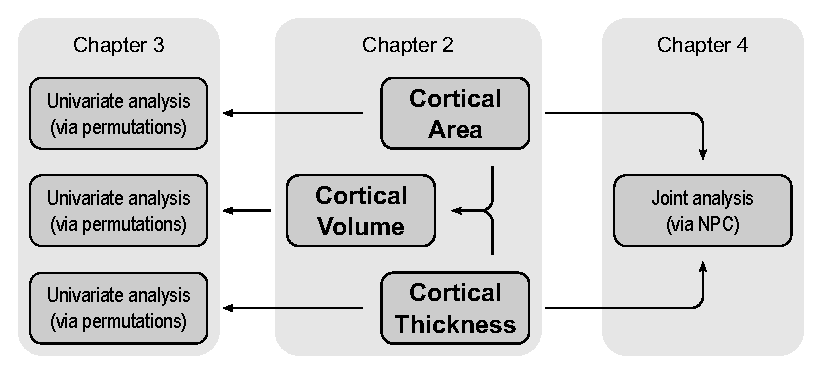
\includegraphics{images/flow.eps}}
\end{center}
\caption[The three ]{Inter-subject comparisons of cortical area and other areal quantities, such as volume, that depends on both area and thickness, use the methods proposed in Chapter~\ref{sec:areal}. Univariate statistical analysis of each of these separately use the strategy discussed in Chapter~\ref{sec:perm}. Joint (combined) analysis of area and thickness, that bypass volumes altogether, use the methods proposed in Chapter~\ref{sec:comb}, in particular the non-parametric combination (\textsc{npc}), but also classical multivariate tests.}
\label{fig:intro:flow}
\end{figure}

\section{Methods for areal quantities}

The general strategy for analyses of cortical measurements consists of the generation of a surface-representation of the brain and its subsequent transformation into a sphere. Vertices of this sphere are then shifted along its surface to allow alignment that matches some feature of interest, such as sulcal depth, myelin content, or functional markers. As the alignment is performed, quantities assigned to vertices or faces, such as thickness or area, are carried along these vertices and faces. Once registration is done, these quantities are interpolated to a common grid (mesh), where comparisons between subjects can be performed.  

While methods to study thickness across subjects are available \citep{Fischl2000}, and use interpolation to a common reference grid using methods such as nearest neighbour or barycentric, such interpolation strategies cannot be used for either cortical area itself, nor to other areal quantities, such as cortical volume, as these are not mass-conservative (pycnophylactic). Chapter~\ref{sec:areal} clarifies the distinction between the nature of these measurements, and proposes the use of areal interpolation. This strategy permits quantities to be studied in absolute terms, as opposed to relative to some reference brain. The chapter proposes that areal quantities are analysed directly in the faces of the mesh from which they were computed, instead of resampled to vertices, which halves the resolution.

We demonstrate that areal data do not follow a normal distribution, being better characterised by a mixture of normal and lognormal distributions, in proportions that vary across the brain and possibly according to the scale of measurement. A power transformation can be considered to address lognormality, although a better alternative is to use permutation methods, that not only do not rely on distributional assumptions, but also allow correction for multiple testing and the use of non-standard statistics.

\section{Methods for permutation inference}

Permutation methods can provide exact control of false positives, making only weak assumptions about the data, and have been available in brain imaging for many particular cases \citep{Holmes1996, Nichols2002}, although no implementation for surface-based methods, even less so for facewise data as we have developed, existed in the literature until this work. With the recent availability of fast and inexpensive computing, the main limitation of permutation tests would be a certain lack of flexibility with respect to arbitrary experimental designs, in particular with respect to nuisance variables in the model, as well as repeated measurements. 

In Chapter~\ref{sec:perm} we report on results on approximate permutation strategies that are more flexible with respect to experimental designs that include such nuisances. We review the literature and conduct detailed simulations to identify the best method for settings that are typical for imaging research. A generic framework for permutation inference for complex general linear models (\textsc{glm}s) when the errors are exchangeable and/or have a symmetric distribution, is presented. Even in the presence of nuisance effects, these permutation inferences are powerful and provide control of false positives in a wide range of common and relevant imaging research scenarios.

We also demonstrate how the inference on \textsc{glm} parameters, originally intended for independent data, can be used in certain special but useful cases in which independence is violated, by means of using exchangeability blocks, that is, sets of observations with shared non-independence, and that can sometimes be treated as a single unit for permutation, i.e., shuffled as a whole, or sometimes serve as delimiters such that permutations happen only within block. The definition of exchangeability blocks allow for groups of observations with same variances, either known or assumed, thus requiring a statistic that preserves certain desirable properties for control of multiple testing even under such scenarios. We provide such a statistic, dubbed $G$-statistic, which is a generalisation of the $F$-statistic, as well as others.

\section{Methods for joint permutation inference}

While gray matter volume can be studied directly using the methods discussed in Chapter~\ref{sec:areal}, it may be the case that true effects affecting thickness and area in opposite directions may cancel each other out. Yet, analysing them separately using univariate methods as in Chapter~\ref{sec:perm} may not aggregate power from having effects acting the two simultaneously. Likewise, participants of an imaging study are often subjected to the acquisition of more than one imaging modality. These modalities are often analysed separately. However, a joint analysis have potential to answer more complex questions and to increment power. Moreover, even a single modality can sometimes be partitioned into subcomponents that disentangle different aspects of brain structure or function. Examples include independent component analysis, as well as scalar measurements from diffusion-tensor imaging. 

In Chapter~\ref{sec:comb} we show how permutation methods can be applied to combination analyses such as those that include multiple imaging modalities, multiple data acquisitions of the same modality, or simply multiple hypotheses on the same data. Using the well-known definition of union-intersection tests and closed testing procedures, we use synchronised permutations to correct for such multiplicity of tests, allowing flexibility to integrate imaging data with different spatial resolutions, surface and/or volume-based representations of the brain, including non-imaging data. 

In particular for the problem of joint inference, we propose and evaluate a modification of the recently introduced Non-Parametric Combination (\textsc{npc}) methodology \citep{Pesarin2010}, such that instead of a two-phase algorithm and large data storage requirements, the inference can be performed in a single phase, with reasonable computational demands. We also evaluate, in the context of permutation tests, various combining methods that have been proposed in the past decades, and identify those that provide the best control over error rate and power across a range of situations. We show that one of these, the method of \citet{Tippett1931}, provides a link between correction for the multiplicity of tests and their combination.

Finally, we discuss how the correction can solve certain problems of multiple comparisons in common designs, and how the combination is distinguished from conjunctions, even though both can be assessed using permutation tests. We also provide a common algorithm that accommodates combination and correction.